\documentclass[a4paper,12pt]{article}
\usepackage{amsmath,amssymb,amsfonts,amsthm}
\usepackage{tikz}
\usepackage [utf8x] {inputenc}
\usepackage [T2A] {fontenc} 
\usepackage[russian]{babel}
\usepackage{cmap} 
\usepackage{gensymb}

% Так ссылки в PDF будут активны
\usepackage[unicode]{hyperref}

% вы сможете вставлять картинки командой \includegraphics[width=0.7\textwidth]{ИМЯ ФАЙЛА}
% получается подключать, как минимум, файлы .pdf, .jpg, .png.
\usepackage{graphicx}
% Если вы хотите явно указать поля:
\usepackage[margin=1in]{geometry}
% Или если вы хотите задать поля менее явно (чем больше DIV, тем больше места под текст):
% \usepackage[DIV=10]{typearea}

\usepackage{fancyhdr}

\newcommand{\bbR}{\mathbb R}%теперь вместо длинной команды \mathbb R (множество вещественных чисел) можно писать короткую запись \bbR. Вместо \bbR вы можете вписать любую строчку букв, которая начинается с '\'.
\newcommand{\eps}{\varepsilon}
\newcommand{\bbN}{\mathbb N}
\newcommand{\dif}{\mathrm{d}}

\newtheorem{Def}{Определение}


\pagestyle{fancy}
\makeatletter % сделать "@" "буквой", а не "спецсимволом" - можно использовать "служебные" команды, содержащие @ в названии
\fancyhead[L]{\footnotesize Термодинамика и молекулярная физика}%Это будет написано вверху страницы слева
\fancyhead[R]{\footnotesize ФМХФ МФТИ}
\fancyfoot[L]{\footnotesize \@author}%имя автора будет написано внизу страницы слева
\fancyfoot[R]{\thepage}%номер страницы —- внизу справа
\fancyfoot[C]{}%по центру внизу страницы пусто

\renewcommand{\maketitle}{%
	\noindent{\bfseries\scshape\large\@title\ \mdseries\upshape}\par
	\noindent {\large\itshape\@author}
	\vskip 2ex}
\makeatother
\def\dd#1#2{\frac{\partial#1}{\partial#2}}


\title{2.4.1 \\ Определение теплоты испарения жидкости} 
\author{Егор Берсенев} 
\date{22 марта 2016 г.}

\begin{document}
	\maketitle
	\section{Цель:}
	\begin{enumerate}
		\item Измерение давления насыщенного пара жидкости при разной температуре.
		\item Вычисление по полученным данным теплоты испарения с помощью уравнения Капейрона-Клаузиуса.
	\end{enumerate}
	\section{Оборудование:}
		Термостат, герметичный сосуд, заполненный исследуемой жидкостью, отсчетный микроскоп.
	\section{Теоретическая часть}
	Испарением называется переход вещества из жидкого состояния в газообразное. Оно происходит на свободной поверхности жидкости. При испарении с поверхности жидкости вылетают молекулы, образуя над ней пар. Для выхода из жидкости молекулы должны обладать достаточной кинетической энергией, т.к. нужна энергия для преодоления сил молекулярного сцепления и совершения работы против внешнего давления. Переход части молекул в пар приводит к охлаждению жидкости. Теплоту парообразования жидкостей можно измерить непосредственно калориметром, однако в работе применем метод, основанный на формуле Клапейрона-Клаузиуса.
	\begin{equation}
		\frac{\dif P}{\dif T} = \frac{L}{T\left(V_2-V_1\right)}
	\end{equation}
	$P$ --- давление насыщенного пара жидкости при температуре $T$, $T$ --- абсолютная температура жидкости и пара, $L$ --- теплота испарени жидкости, $V_2$ --- объем пара, $V_1$ --- объем жидкости. При малом давлении можно пренебречь объемом жидкости
	Также пренебрежем коэффициентами Ван-дер-Ваальса и будем пользоваться уравнением состояния идеального газа.
	\begin{equation}
		V  = \frac{RT}{P}
	\end{equation}
	Разрешим относительно $L$.
	\begin{equation}
		L = \frac{RT^2}{P}\frac{\dif P}{\dif T} = -R\frac{\dif\left(\ln P\right)}{\dif\left( 1/T \right)}
	\end{equation}
	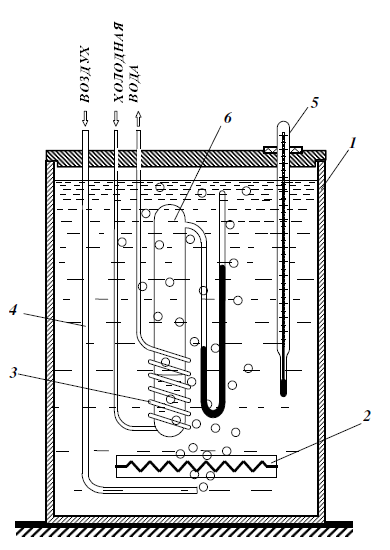
\includegraphics[width = 0.4\linewidth]{instrument}
	
	На рисунке изображена экспериментальная установка. Наполненный водой резервуар 1 ирает роль термостата. Нагревание термостата производится спиралью 2, подогревамое электрическим током. Для охлаждения воды в термостате через змеевик 3 пропускается холодная вода. Вода в термостате перемешивается воздухом, поступающим через трубку 4. Температура воды измерятется термометром 5. В термостат погружен запаянный прибор 6 с исследуемой жидкостью.
	Давление насыщенного пара определяется по ртутному манометру.
	\section{Практическая часть}
		Включим нагревание. Проведем измерения в диапазоне температур от 8\celsius до 30\celsius.
		\begin{center}
			\begin{tabular}{|l|l|l|l|}
				T, \celsius      & 1/T  & H, см    & P,  Па    \\ \hline
				281.15 & 3.56 & 1.74 & 2319 \\
				283.45 & 3.53 & 1.91 & 2546 \\
				286.35 & 3.49 & 2.22 & 2959 \\
				289.55 & 3.45 & 3    & 3998 \\
				292.15 & 3.42 & 3.65 & 4865 \\
				295.35 & 3.39 & 4.2  & 5598 \\
				298.25 & 3.35 & 5.03 & 6704 \\
				301.15 & 3.32 & 5.94 & 7917 \\
				303.15 & 3.30 & 6.72 & 8956 \\ \hline
				297.15 & 3.36 & 4.67 & 6224 \\
				298.95 & 3.37 & 4.07 & 5424 \\
				293.15 & 3.41 & 3.60 & 4798 \\
				290.95 & 3.44 & 3.20 & 4265 \\
				289.15 & 3.46 & 2.59 & 3452 \\
				286.35 & 3.49 & 2.38 & 6172 \\ \hline
			\end{tabular}
		\end{center}
	\begin{center}
		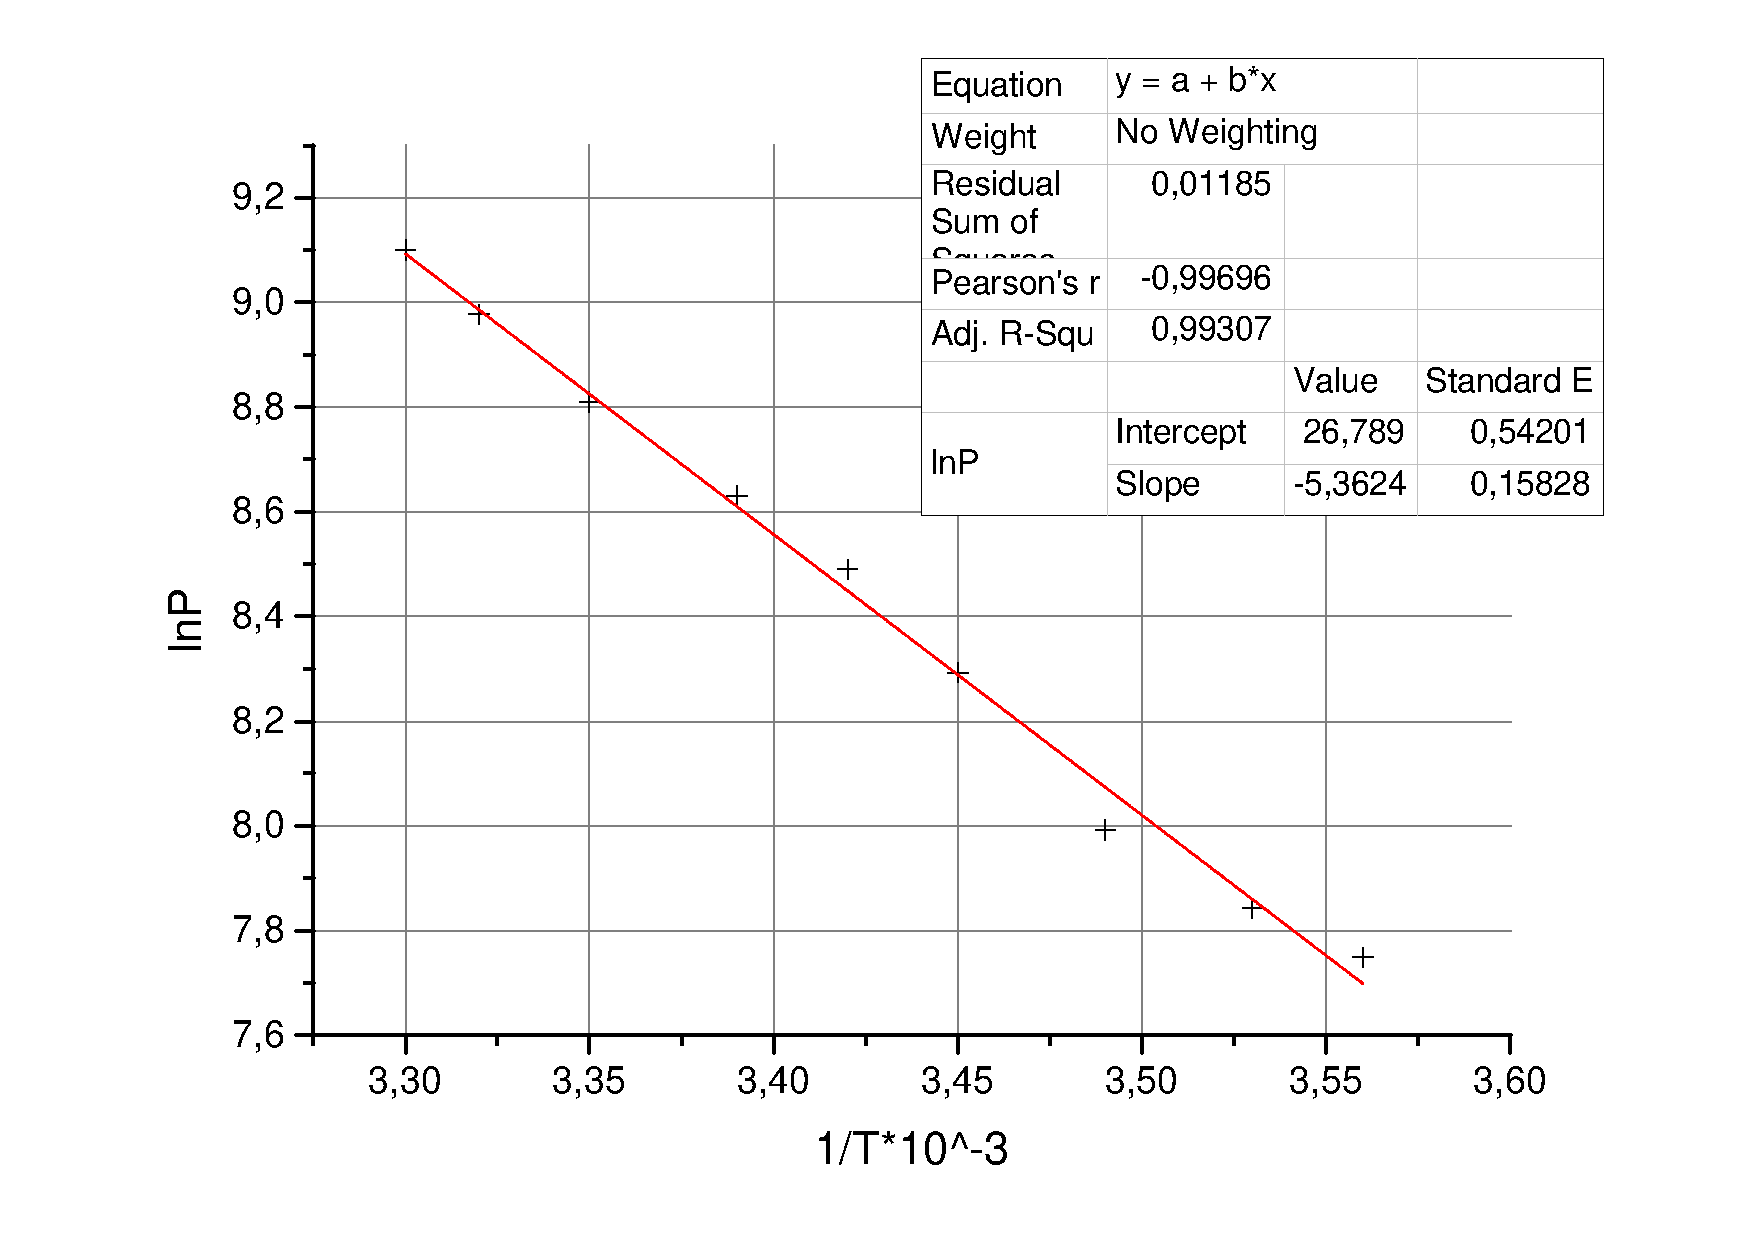
\includegraphics[width = 0.7\linewidth]{up}
		
		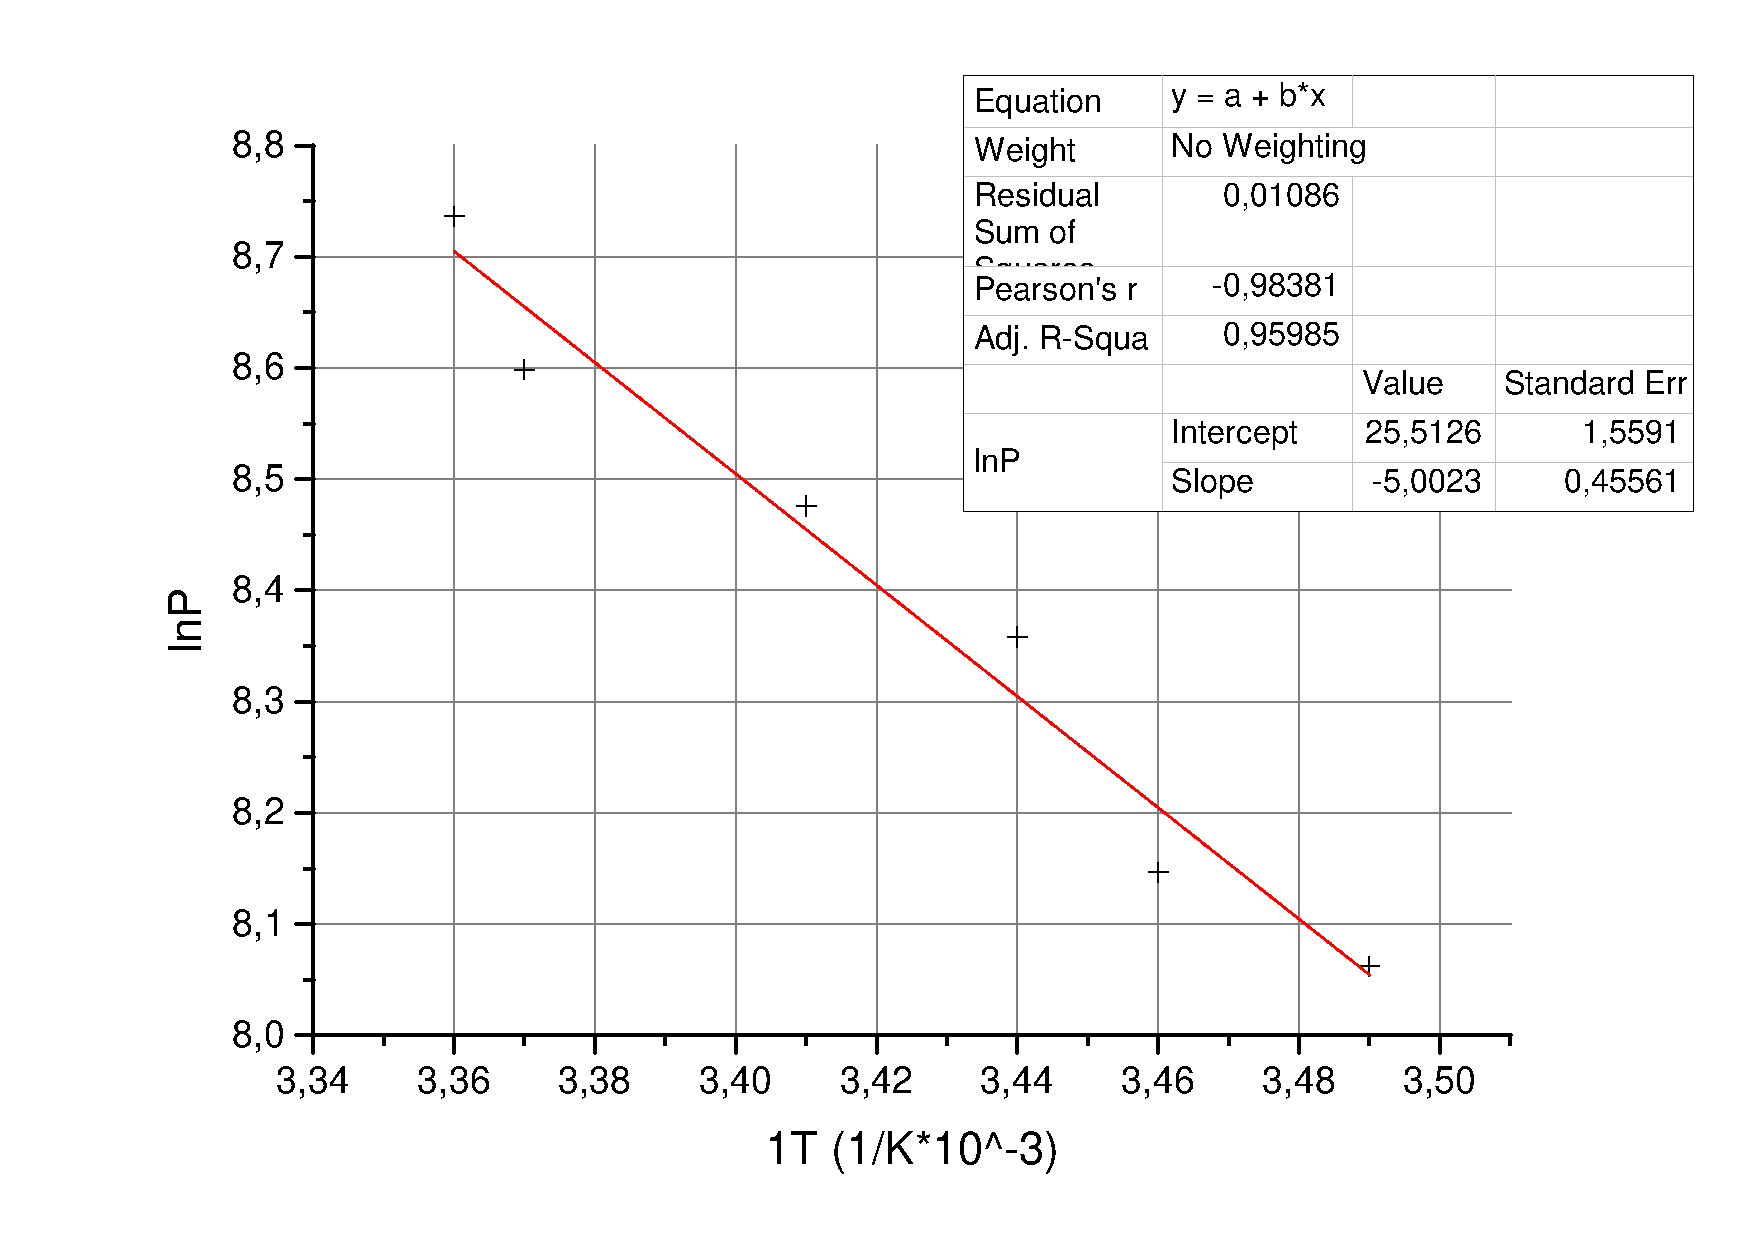
\includegraphics[width = 0.7\linewidth]{down}
	\end{center}
	По формуле получим значение теплоты испарения.
		$L = -R\frac{\dif\left(\ln P\right)}{\dif\left( 1/T \right)} = \left(44.58 \pm 1.32\right)  \frac{\text{кДж}}{\text{моль}}$
		Табличное значение --- $42\, \frac{\text{кДж}}{\text{моль}}$.
		Результат сходится с табличным почти в пределах погрешности.
	\section{Вывод}
	С помощью уравнения Клапейрона-Клаузиуса можно измерять теплоту парообразования жидкости. Однако, экспериментальная установка не лишена недостатков: так, например к искажению результатов опыта привела недостаточная пермешиваемость жидкости и сильная переохлажеденность. 
\end{document}


